
\begin{figure}[!tbh]
  \centering
  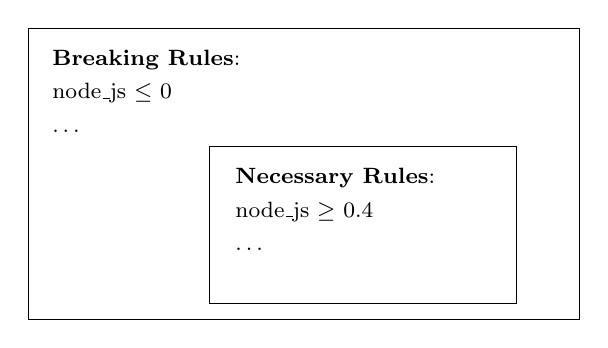
\begin{tikzpicture}
    \draw (0,0) rectangle (7,3.7); 
    \node [align=left] at (1.5,2.9) {\footnotesize \textbf{Breaking Rules}: \\ \footnotesize node\_js $\le$ 0 \\ \footnotesize \ldots};
    \draw (2.3,0.2) rectangle (6.2,2.2);
    \node [align=left] at (3.9,1.4) {\footnotesize \textbf{Necessary Rules}: \\ \footnotesize node\_js $\ge$ 0.4 \\ \footnotesize \ldots};
  \end{tikzpicture}
  \caption{An example set of necessary and breaking rules if we have seen a failing file with {\footnotesize node\_js: 0}, and a passing file with {\footnotesize node\_js: 0.4.}}
  \label{fig:versionSL}
\end{figure}
